\documentclass[a4paper, 12pt]{article}
\usepackage{graphicx}
\usepackage{amsmath}
\usepackage{hyperref}
\usepackage{float}

\title{Logistic Regression using Gradient Descent}
\author{Le Duc Bach -- ICT.2440039}
\date{\today}

\begin{document}

\maketitle

\section{Introduction}
Logistic regression is a widely used method for binary classification tasks. This report details an implementation of logistic regression using gradient descent optimization in Python. The goal is to classify data based on two input features extracted from a dataset named \texttt{loan.csv}.

\section{Methodology}

\subsection{Data Processing}
The dataset contains three columns: two continuous features ($x_1$ and $x_2$), and one binary target label $y$. The CSV file is read line by line to extract these values into Python lists.

\subsection{Model Formulation}
Logistic regression models the probability of class $y = 1$ using the sigmoid function:

\[
P(y=1 \mid x) = \sigma(w_1 x_1 + w_2 x_2 + w_0), \quad \text{where } \sigma(z) = \frac{1}{1 + e^{-z}}
\]

The loss function used is the average negative log-likelihood:

\[
J(w_0, w_1, w_2) = -\frac{1}{N} \sum_{i=1}^N \left[ y_i (w_1 x_{i1} + w_2 x_{i2} + w_0) - \log(1 + e^{w_1 x_{i1} + w_2 x_{i2} + w_0}) \right]
\]

\subsection{Gradient Descent}
The weights are optimized using batch gradient descent. The partial derivatives of the loss function with respect to each weight are calculated and used to update weights iteratively:

\begin{align*}
\frac{\partial J}{\partial w_0} &= \frac{1}{N} \sum_{i=1}^N \left(1 - y_i - \sigma(-z_i)\right) \\
\frac{\partial J}{\partial w_1} &= \frac{1}{N} \sum_{i=1}^N \left( -y_i x_{i1} + x_{i1}(1 - \sigma(-z_i)) \right) \\
\frac{\partial J}{\partial w_2} &= \frac{1}{N} \sum_{i=1}^N \left( -y_i x_{i2} + x_{i2}(1 - \sigma(-z_i)) \right)
\end{align*}

Where $z_i = w_1 x_{i1} + w_2 x_{i2} + w_0$.

\subsection{Hyperparameters}
\begin{itemize}
    \item Learning rate ($\eta$): 0.9
    \item Number of iterations: 10,000
    \item Initial weights: $w_0 = 0$, $w_1 = 1$, $w_2 = 2$
\end{itemize}

\section{Results}

\subsection{Decision Boundary}
After training, the decision boundary separating the two classes was computed using the equation:

\[
x_2 = -\frac{w_0 + w_1 x_1}{w_2}
\]

\begin{figure}[H]
    \centering
    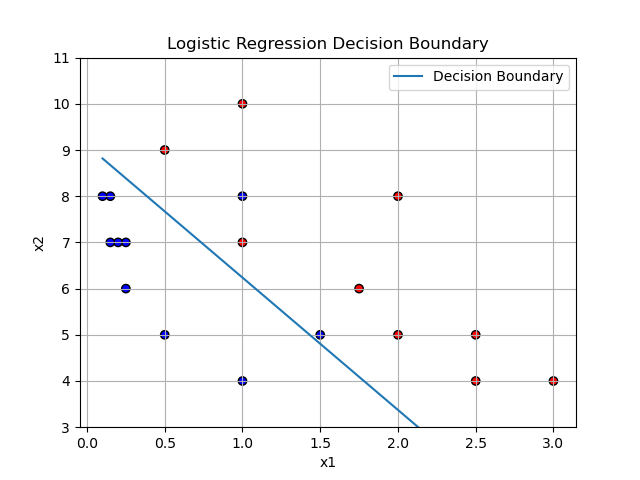
\includegraphics[width=0.7\textwidth]{Figure_1.png}
    \caption{Decision Boundary of the Logistic Regression Model}
\end{figure}

\subsection{Loss Curve}
The loss function decreased significantly and stabilized as training progressed, indicating successful convergence of the model.

\begin{figure}[H]
    \centering
    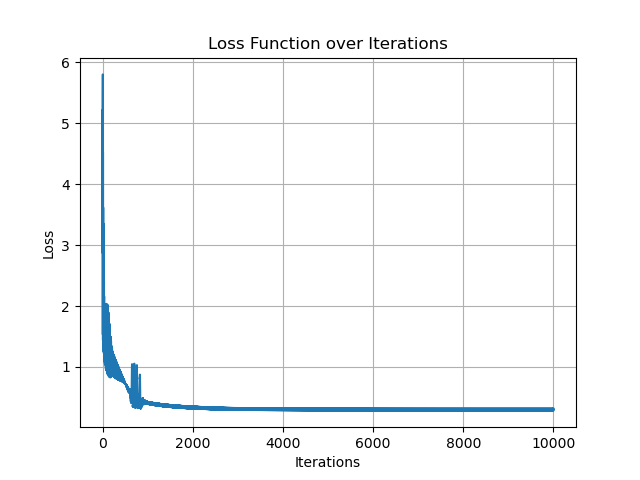
\includegraphics[width=0.7\textwidth]{Figure_2.png}
    \caption{Loss Function over Iterations}
\end{figure}

\section{Conclusion}
The logistic regression model was successfully trained using batch gradient descent. The loss curve shows effective learning, and the decision boundary indicates that the model can separate the two classes based on the given features. This experiment demonstrates a fundamental approach to implementing logistic regression from scratch using Python.

\end{document}
